We are interested in examining the performance of algorithms to compute minimal IVCs.
We examine \textbf{Grow-Shrink}, the algorithm presented in Section \ref{sec:onaivc}, and the two state-of-the-art algorithms: \textbf{Offline MARCO} (\aivcalg Section \ref{sec:offaivc}), and \textbf{Online MARCO} (Section \ref{sec:onaivc}) that performs a shrink step prior to returning a solution to ensure minimality.
%\old{We examine three algorithms:
%\textbf{Offline MARCO}, the algorithm from~\cite{Ghass17AllIVCs}, \textbf{Online MARCO}, a variant of the algorithm from~\cite{Ghass17AllIVCs} that performs a shrink step prior to returning a solution to ensure minimality, and \textbf{Grow-Shrink}, the algorithm described in this paper.}
We investigate the following research questions:
\begin{itemize}
  \item \textbf{RQ1:} For the large models where the complete MIVC enumeration is intractable,
how many MIVCs are found within the given time limit?
  \item \textbf{RQ2:} For the tractable models, i.e., models in which all MIVCs are found, how much time is required to complete the enumeration of MIVCs?
  \item \textbf{RQ3:} Finally, we are interested in how many solver calls are necessary for the enumeration. What is the (average) number of solver calls with result adequate/inadequate required by evaluated online algorithms to produce individual MIVCs?
\end{itemize}

\subsection{Experimental Setup}
  We start from a benchmark suite that is a superset of the benchmarks used in the previous experiments. This suite contains 660 models, and includes all models that yield a valid result (530 in total) from previous Lustre model checking papers~\cite{Hagen08:FMCAD,piskac2016} and 130 industrial models yielding valid results derived from an infusion pump system \cite{hilt2013} and other sources \cite{piskac2016,NFM2015:backes}.
As this paper is concerned with analysis problems involving multiple MIVCs, we include only models that had more than 4 MIVCs (46 models in total).  To consider problems with many IVCs, we took those models and mutated them, constructing 20 mutants for each model. The mutants varied both in the number and in the size of individual MIVCs.
We added the mutants that still yielded valid results and have more than 5 MIVCs (384 in total) back to the benchmark suite.
Thus, the final suite contains 430 Lustre models. The original benchmarks and our augmented benchmark are available online\footnote{\url{https://github.com/elaghs/benchmarks}}.
%\cite{bench}.

For each test model, we configured \texttt{JKind} to use the \texttt{Z3} solver and the ``fastest'' mode of \texttt{JKind} (which involves running the $k$-induction and PDR engines in parallel and terminating when a solution is found). The experiments were run on a  3.50GHz  Intel(R) i5-4690 processor 16 GB memory machine running Linux with a 30 minute timeout.  All experimental data is available online\footnote{\url{https://github.com/jar-ben/online-mivc-enumeration}}.
%~\cite{expr}.




\begin{figure*}
\centering
\begin{minipage}{\textwidth}
\centering
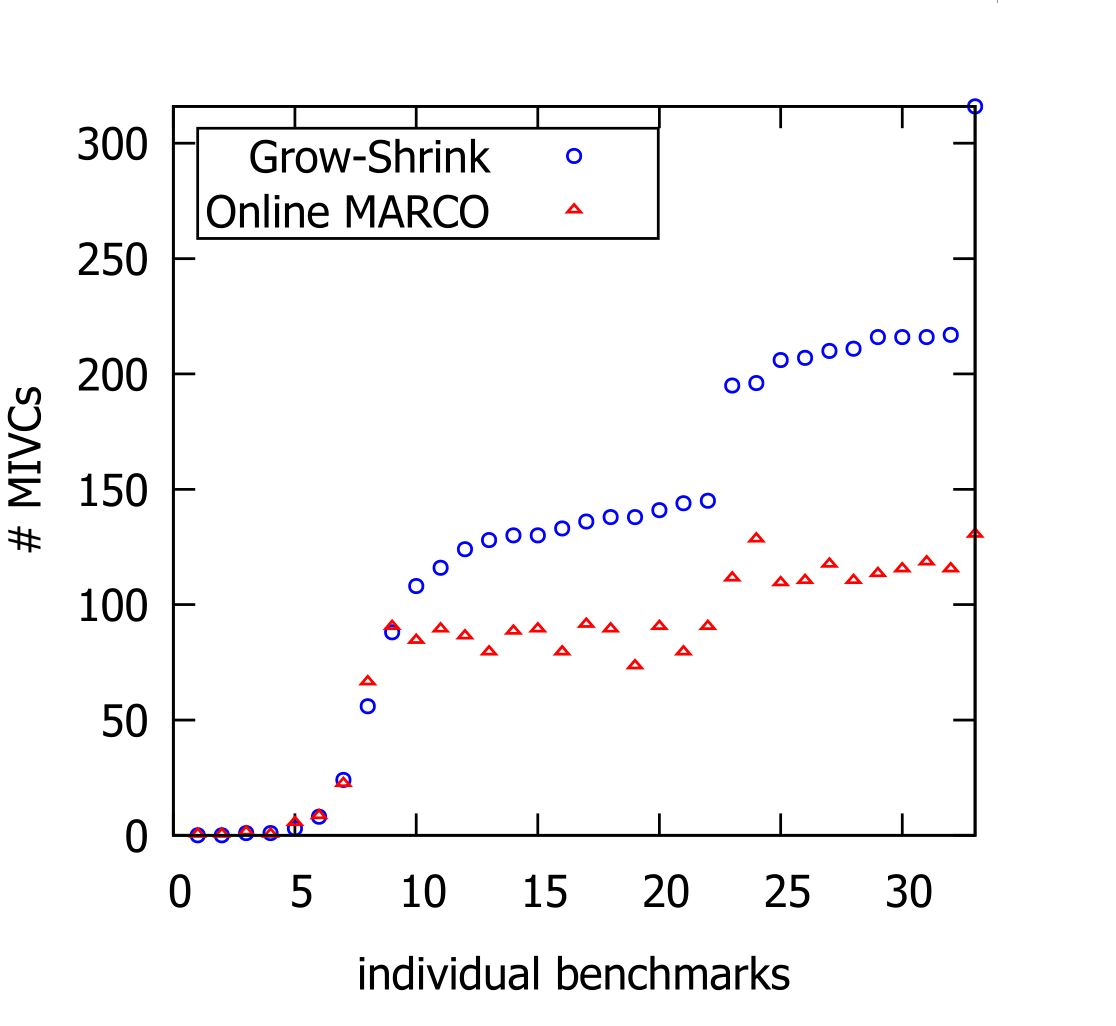
\includegraphics[scale=0.5]{./figs/found_mivcs.png}%
\captionof{figure}{Number of MIVCs produced by online algorithms.}%
\label{res:found_mivcs}
\end{minipage}\hfill
\begin{minipage}{\textwidth}
\centering
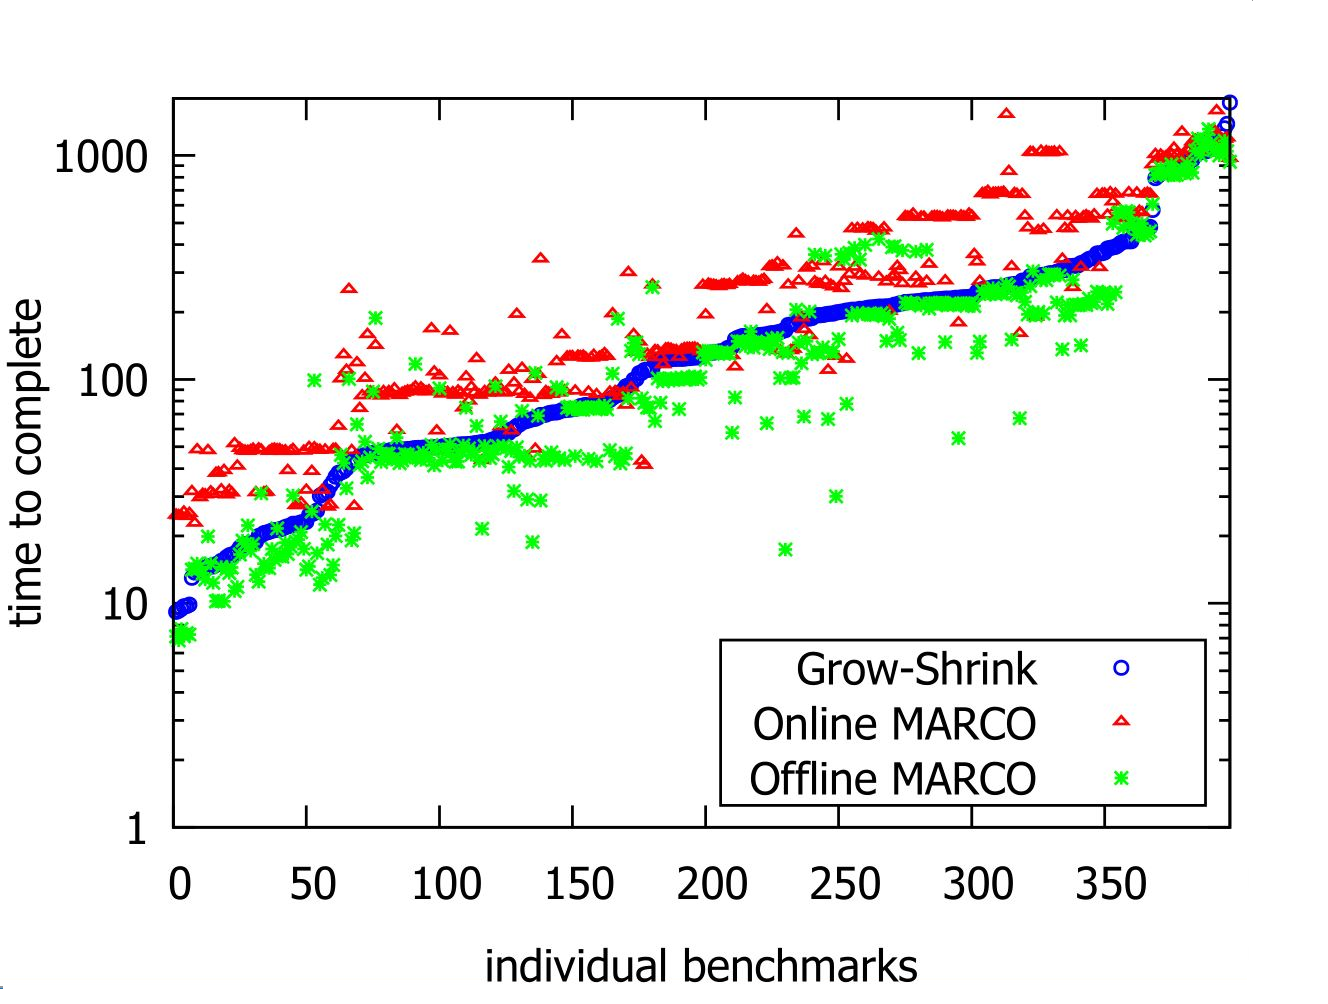
\includegraphics[scale=0.5]{./figs/time_to_complete.png}%
\captionof{figure}{Runtime for tractable benchmarks for all algorithms in a log scale.}%
\label{res:time_to_complete}
\end{minipage}
\end{figure*}



\subsection{Experimental Results}
In this section, we examine the experimental results to address the research questions.

%\vspace{-5pt}

\subsubsection{RQ1 and RQ2}
Data related to the first two research questions are shown in Figures~\ref{res:found_mivcs} and~\ref{res:time_to_complete}.
Figure~\ref{res:found_mivcs} describes the number of MIVCs found be the two online algorithms in the intractable benchmarks, i.e., the benchmarks where the algorithms did not complete the computation within the time limit. There are 33 such benchmarks. The Grow-Shrink substantially outperforms Online MARCO in the majority of the benchmarks, finding an average of 55\% additional MIVCs.

Figure~\ref{res:time_to_complete} describes the time for each algorithm needed to complete the computation in the case of 397 tractable benchmarks.

Grow-Shrink is on
average only 1.08 times slower than Offline MARCO,
yet as previously discussed,
has the advantage of returning guaranteed MIVCs,
rather than approximate MIVCs.
It is on average 1.50 times faster than Online MARCO.


%It is much faster than the Online MARCO algorithm.


%\vspace{-5pt}

\subsubsection{RQ3}  For RQ3, we examined the number of required calls to the solver per MIVC.  For this question, we used the 33 models that contained a large number of MIVCs ($>$70) in order to show the solver efficiency as the number of MIVCs increased.  A point with coordinates $(x,y)$ states that the algorithm needed to perform $y$ solver calls (on average) in order to produce the first $x$ MIVCs. We grouped the calls in terms of the number of calls that returned {\em adequate} vs. {\em inadequate} results.  It is evidenced by the results in Figure~\ref{res:checks}, the new algorithm improves upon Online MARCO as the number of MIVCs becomes larger.

\begin{figure*}
\centering
\begin{subfigure}{\textwidth}
  \centering
  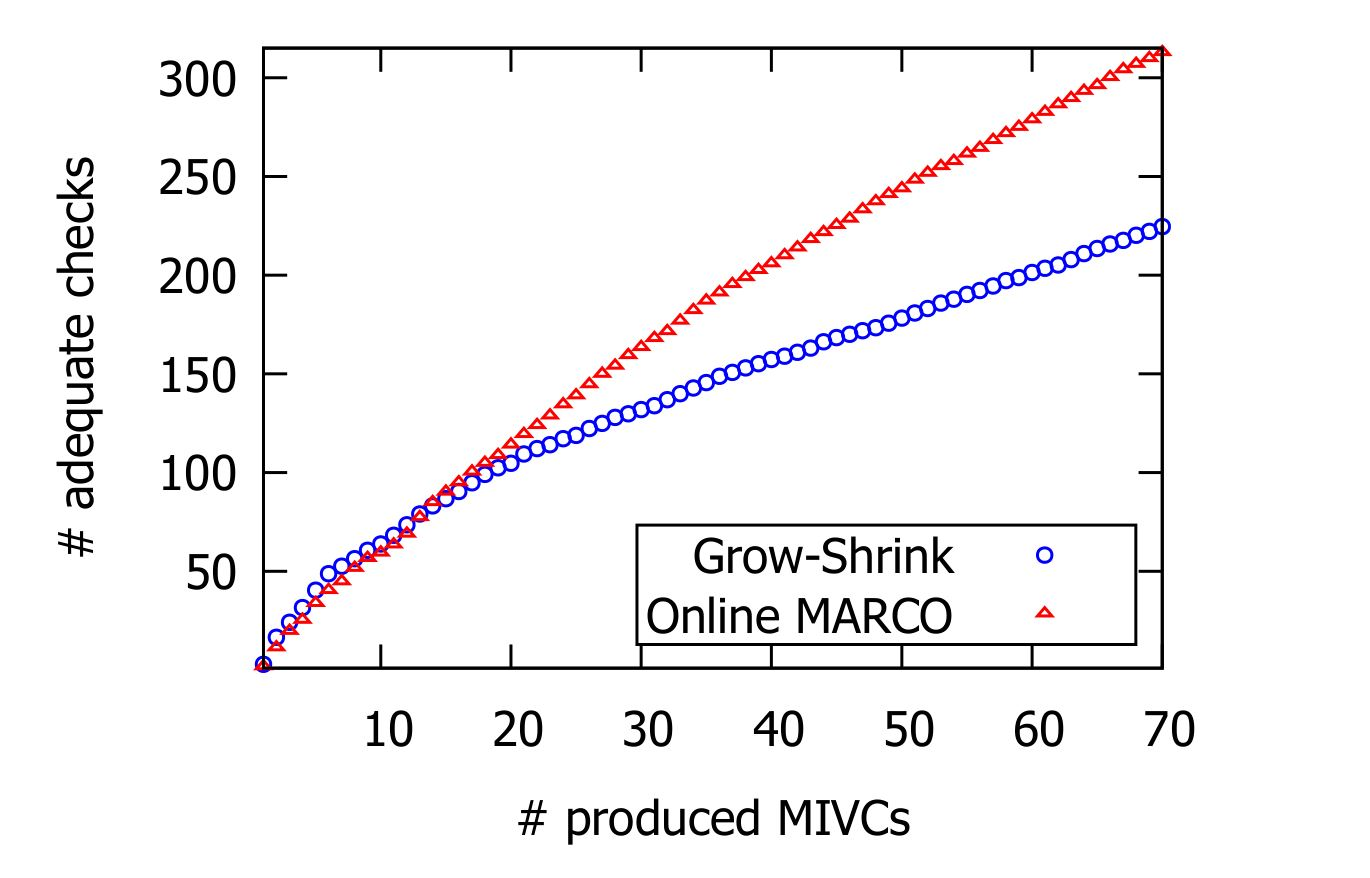
\includegraphics[scale=0.5]{./figs/adequate_checks_per_mivc_70.png}
  \caption{Checks with result ``adequate''}
  \label{res:adequate_checks}
\end{subfigure}\hfill
\begin{subfigure}{\textwidth}
  \centering
  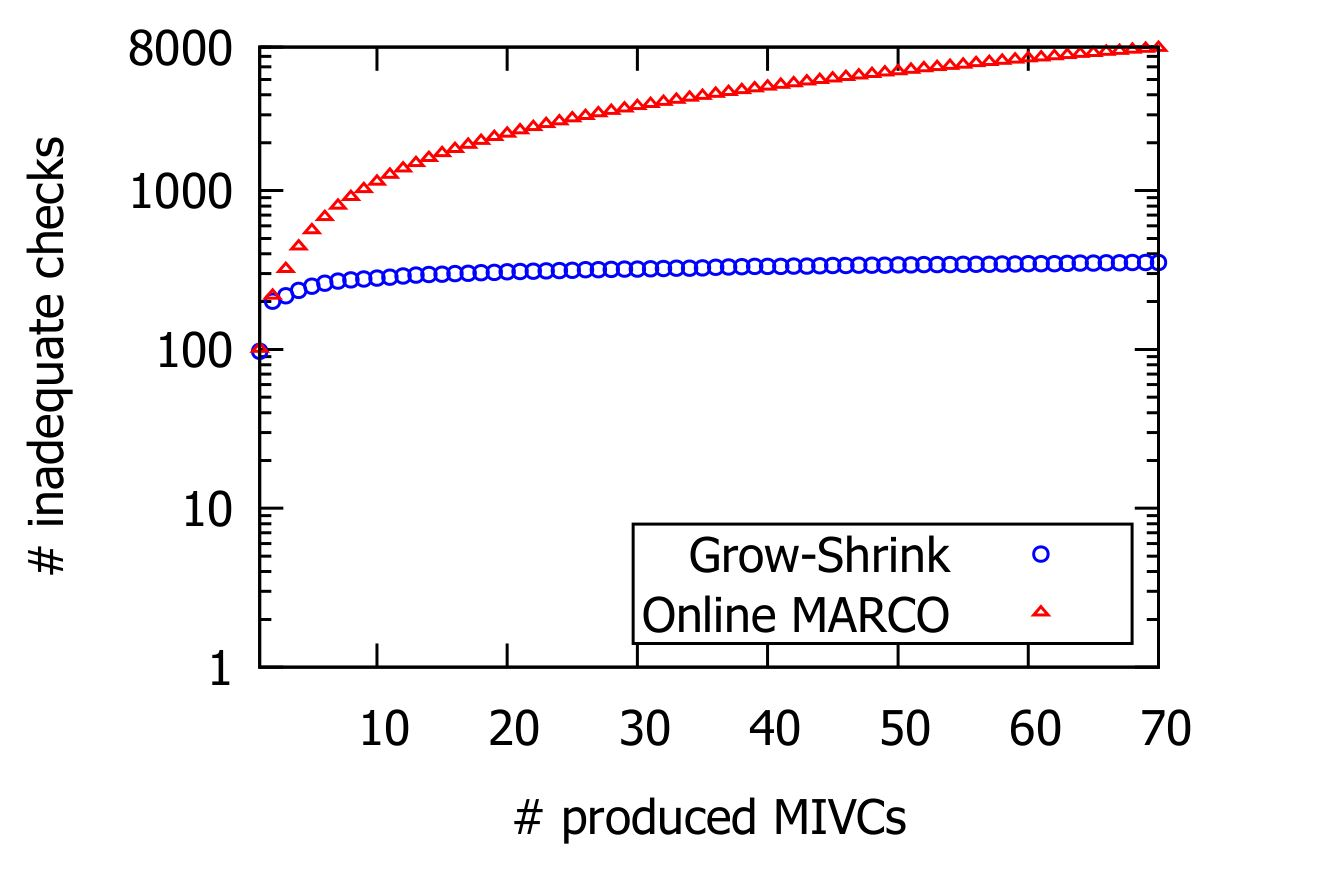
\includegraphics[scale=0.5]{./figs/inadequate_checks_per_mivc_70.png}
  \caption{Checks with result ``inadequate''}
  \label{res:inadequate_checks}
\end{subfigure}
\caption{Average number of performed adequacy checks required to produce individual MIVCs. Note that Figure (b) is in a log scale.}
\label{res:checks}
\end{figure*}

The improvement in the number of \emph{inadequate} calls is due the novel shrinking and growing procedures.
Each (approximately) maximal inadequate subset found by the growing procedure allows to save (up to exponentially) many inadequate calls during subsequent executions of the shrinking procedure.
Indeed, the Grow-Shrink algorithm performed on average only 353 inadequate calls to output the first 70 MIVCs, whereas the online MARCO needed to perform 7775 calls to output the same number of MIVCs.

The improvement in the number of \emph{adequate} calls is not so significant as in the case of inadequate calls. Yet, since the adequate calls are usually much more time consuming than inadequate ones, even a slight saving in the number of adequate calls might significantly speed up the whole computation. The Grow-Shrink algorithm saves adequate calls due to the usage of the shrinking queue and due to the invariants that are maintained by the queue. In particular, shall two comparable sets appear in the queue, only the smaller is left. Thus, the algorithm avoids shrinking of relatively large sets and saves some adequate calls.
